\documentclass[a4paper, 10pt]{article}

% Typography & Font Handling
%\usepackage[utf8]{inputenc}
\usepackage[T1]{fontenc}
\usepackage{lmodern}
\usepackage{microtype}
\usepackage{fontspec}
\usepackage{sectsty}
\usepackage{fixltx2e}
\usepackage{titlesec}

% Fonts
%\usepackage{garamondlibre}
\setmainfont{Garamond Libre}  % Serif
\setsansfont{TeX Gyre Heros}    % Sans
\setmonofont{TeX Gyre Cursor}  % Mono

% Mathematics
\usepackage{amsmath}
\usepackage{amssymb}
\usepackage{mathtools}

% Numbers
\usepackage{siunitx}
\sisetup{
    detect-all,   % detects the surrounding font
    detect-family,
    detect-shape,
    detect-weight
}

% Lists
\usepackage{enumitem}

% Tables
\usepackage{booktabs}
\usepackage{array}
\usepackage{tabularx}
\newcolumntype{Y}{>{\raggedright\arraybackslash}X}

% Graphics
\usepackage{graphicx}
\usepackage{float}

% Figures
\usepackage{subcaption}
\usepackage{wrapfig}

% Circuits
\usepackage{circuitikz}

% Code Listings
\usepackage{listings}

% Layout & Page Formatting
\usepackage{geometry}
\usepackage{fancyhdr}
%\usepackage{indentfirst}
\usepackage{parskip}
% References
\usepackage{hyperref}
\usepackage{cleveref}

%\usepackage{lipsum}

%============================================
\geometry{
headheight=25pt,
top=1in,
bottom=1in,
left=0.5in,
right=0.5in
}
\title{ELEC ENG 2411: Ex template\vspace{5em}
}
\author{
	{\Large Prepared by:}\\
	Lucas Rufkahr\vspace{5em}\\
	%{\Large In Collaboration with:}\\
	%Aiden Burns\vspace{5em}\\
	{\Large Submitted to:}\\
	Sokrat Aldarmini\vspace{5em}\\
	{\Large Submitted on:}\\
	\today
}
\date{}

\titleformat*{\section}{\Large\bfseries\sffamily}
\renewcommand{\thesection}{\arabic{section}}
\titleformat*{\subsection}{\large\bfseries\sffamily}
\renewcommand{\thesubsection}{\thesection.\Alph{subsection}}
\titleformat*{\subsubsection}{\itshape\sffamily}
\renewcommand{\thesubsubsection}{\thesubsection.\roman{subsubsection}}

\begin{document}
\setcounter{secnumdepth}{4}
\pagestyle{fancy}
\fancyhead[L]{Lucas Rufkahr}%, Aiden Burns}
\fancyhead[C]{Template}
\fancyhead[R]{EE2411 --- Section 305\\\today}
\maketitle
\thispagestyle{empty}
%========================
\pagebreak
\section*{Part 1 Step 1}
This step introduces the concept of sampling. First we create a \texttt{unitstep()} function. Then we create a vector \texttt{t = -2:6} using a step size of 1. The we create a vector \texttt{y = unitStep(t)}. We create the plot with circle markers to represent the discrete value at that time. The dashed lines represent the continuous representation.

\section*{Part 1 Step 2}
Now we create a new vector \texttt{t1 = -2:0.1:6}. It is the same interval as before just with a smaller step size. We then create the vector \texttt{y1 = unitStep(t1)}. We use the hold on command to draw this plot on the same figure. The plot for step 1 and step 2 are shown in figure \ref{fig:part1step12}. We calculate this using the formula $\frac{1}{T_{s}} = f_{s}$ where $f_{s}$ is the sampling frequency and $T_{s}$ is the sampling interval.

\begin{figure}[H]
        \centering
        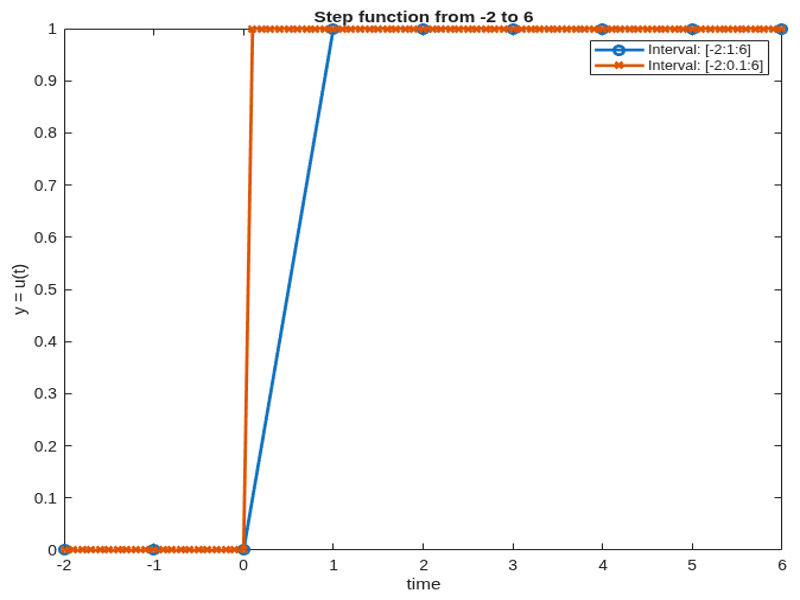
\includegraphics[scale=1]{./assets/part1/part1step2.png}
        \caption{unitStep shown with different sampling sizes.}
        \label{fig:part1step12}
\end{figure}

\section*{Part 1 Step 3}
The sampling data for \texttt{y} and \texttt{y1} are shown in table \ref{tab:part1step3}.

\begin{table}[H]
	\centering
	\begin{tabularx}{0.7\linewidth}{YYY}
		   	    & Sampling Interval & Sampling Frequency \\
		\texttt{y}  & 1		        & 1		     \\
		\texttt{y1} & 0.1	        & 10		     \\	 
	\end{tabularx}
	\caption{Sampling interval and frequency for \texttt{y} and \texttt{y1}.}
	\label{tab:part1step3}
\end{table}

\section*{Part 1 Step 4}
We now create a vector \texttt{t2 = 0:2}. We then create a splot of a 1Hz sine wave with \texttt{y2 = sin(t2 * 2 * pi)}. We then create a new figure and plot the result. We see the plot is of diagonal line. This is because our step size or sampling frequency is too small. The plot for this is shown in \ref{fig:part1step4}.

\begin{figure}[H]
        \centering
        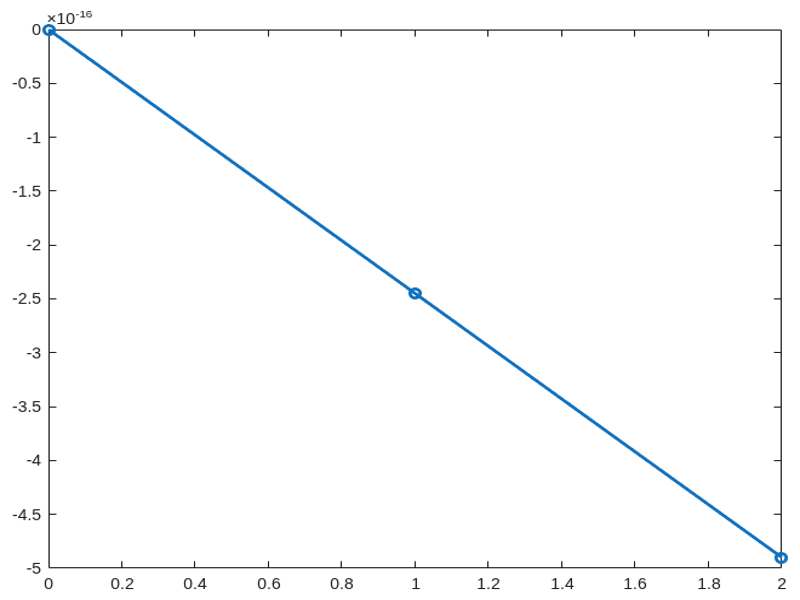
\includegraphics[scale=1]{./assets/part1/part1step4.png}
        \caption{A sinusoid wave with a very low sampling frequency.}
        \label{fig:part1step4}
\end{figure}

\section*{Part 1 Step 5}
We then start decreasing the sampling frequency by a factor of 2. We found that at a sampling frequency of 0.0375, we see a smooth sine wave. We computed the sampling frequency for the smooth sine wave as $26.67$. The smooth sinusoid is shown in \ref{fig:part1step5}.

\begin{figure}[H]
        \centering
        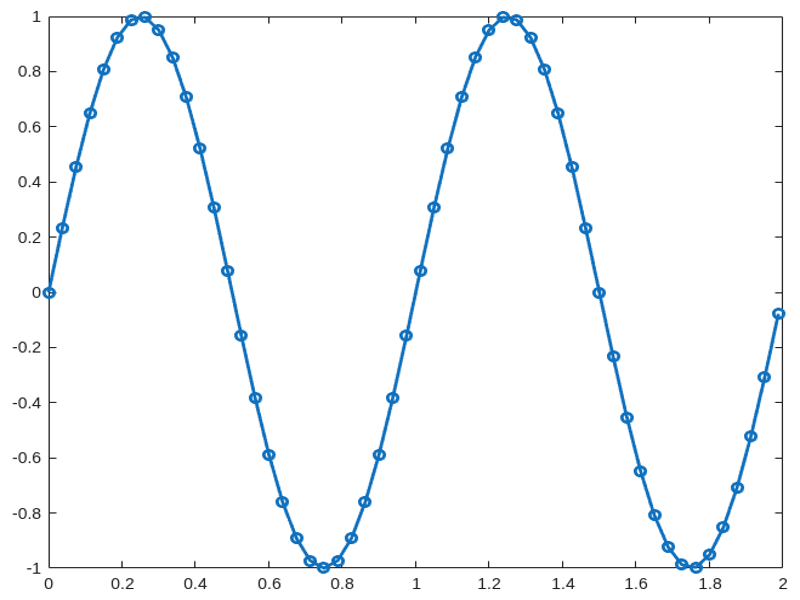
\includegraphics[scale=1]{./assets/part1/part1step5.png}
        \caption{A sinusoid wave with sampling frequency of 26.67.}
        \label{fig:part1step5}
\end{figure}

\section*{Part 2 Step 1}
We begin part 2 by creating a vector \texttt{t = 0:0.1:5}. We then create a vector \texttt{y\_o = 2 * (unitStep(t - 2) - unitStep((t - 2) - 0.5));} which is a rectangular starting at 2 and lasting for 0.5. We then create a new figure and plot the pulse. The plot is shown in figure \ref{fig:part2step1}.

\begin{figure}[H]
	\centering
	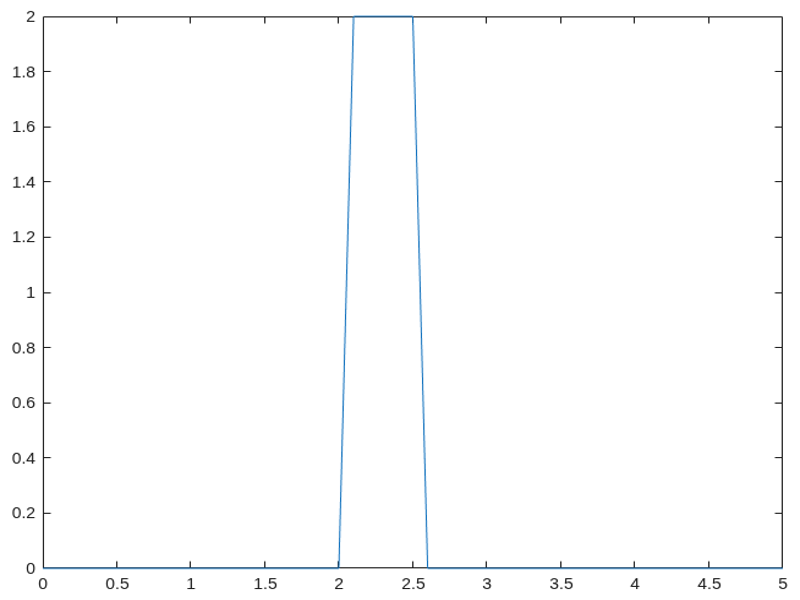
\includegraphics[scale=1]{./assets/part2/part2step1.png}
	\caption{A pulse signal.}
	\label{fig:part2step1}
\end{figure}

\section*{Part 2 Step 2}
This step is where we calculate a convolution of this pulse with itself.

\section*{Part 2 Step 3}
MATLAB can also compute convolution using the function \texttt{conv()}. We create a vector \texttt{y = conv(y\_o,y\_o)} to do the convolution. The plot for the convolution is shown in figure \ref{fig:part2step3}.

\begin{figure}[H]
        \centering
        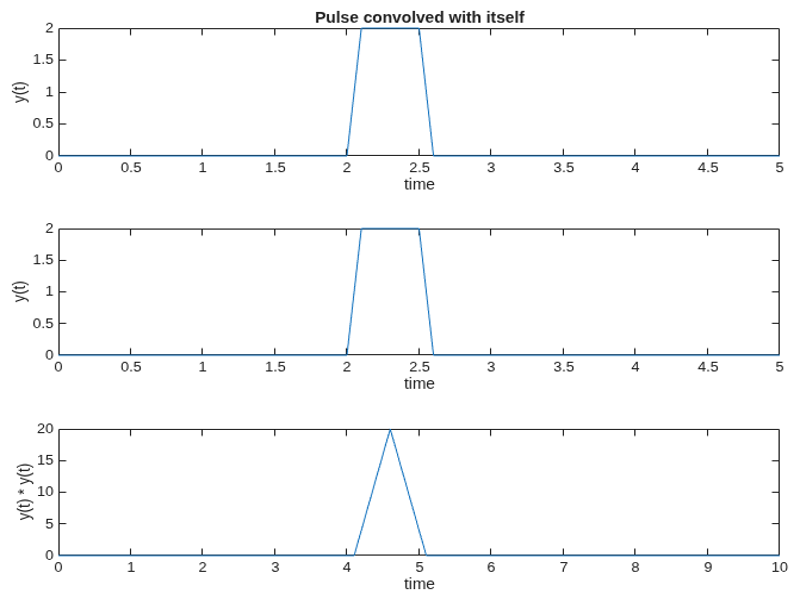
\includegraphics[scale=1]{./assets/part2/part2step3.png}
        \caption{Two identical pulses convolved with each other.}
        \label{fig:part2step3}
\end{figure}

\section*{Part 2 Step 4}
Now we use a time vector \texttt{t = 0:0.01:5}. This is a finer sampling frequency and the output should match more similar to the theoretical geometric calculation. The plot for this is shown in \ref{fig:part2step4}.

\begin{figure}[H]
        \centering
        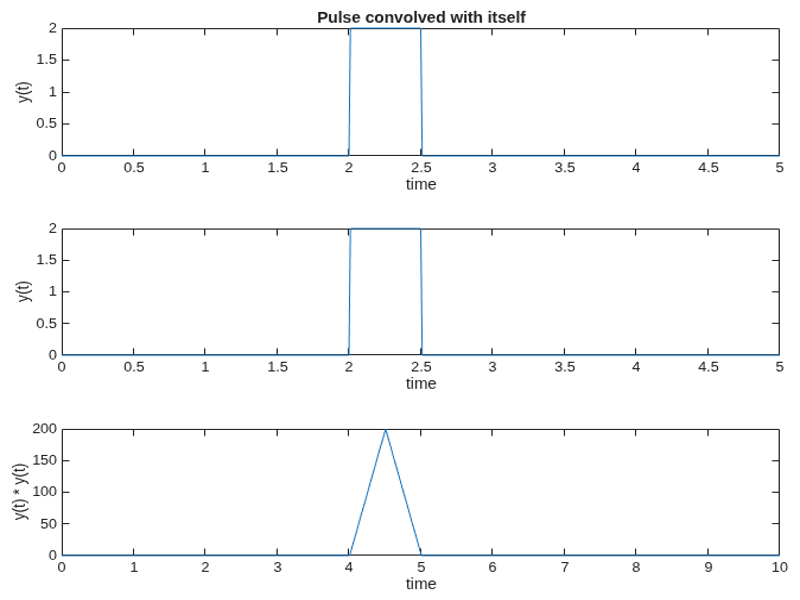
\includegraphics[scale=1]{./assets/part2/part2step4.png}
        \caption{Convolution of two pulses with a sampling frequency of 10Hz.}
        \label{fig:part2step4}
\end{figure}

\section*{Part 2 Step 5}
This time we use a time vector \texttt{t = 0:0.0001:5} which is a sampling frequency of 1000Hz. The plot for this is shown in \ref{fig:part2step5}.

\begin{figure}[H]
        \centering
        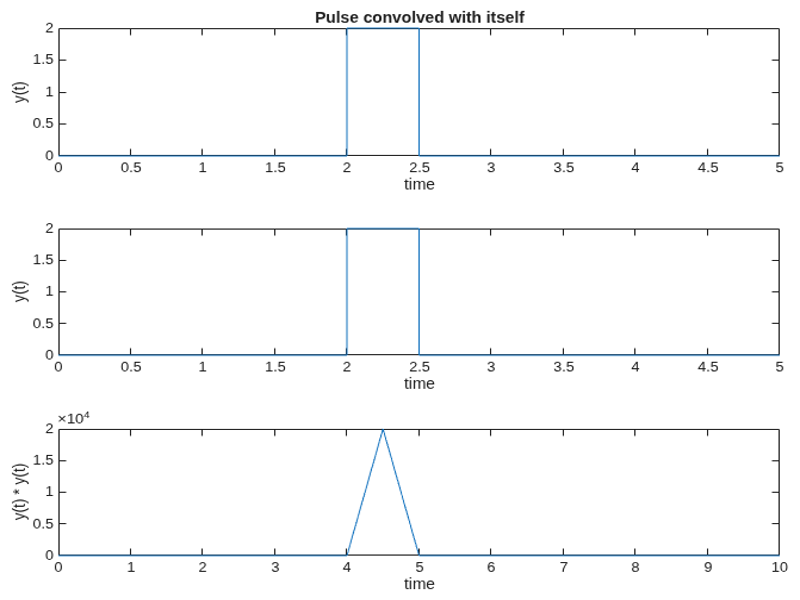
\includegraphics[scale=1]{./assets/part2/part2step5.png}
        \caption{Convolution of two pulses with a sampling frequency of 1000Hz.}
        \label{fig:part2step5}
\end{figure}

\section*{Part 3 Step 1}
We want to consider an RLC circuit expressed as a differential equation. The equation is,
\begin{equation}
	\frac{d^2v(t)}{dt^2} + \frac{R}{L}\frac{dv(t)}{dt} + \frac{1}{LC}v(t) = \frac{1}{LC}x(t)
\end{equation}
with an impulse response of,
\begin{equation}
	h(t) = \frac{\omega^2_n}{\omega_d}e^{-\alpha t}sin(\omega_d t)u(t)
\end{equation}
First we create constants \texttt{R = 63}, \texttt{L = 5e-3} , \texttt{C = 5e-6}, \texttt{alpha = R / (2 * L)}, \texttt{f\_angular\_natural = (sqrt(L * C))\^{}(-1)}, \texttt{f\_angular\_d = sqrt(f\_angular\_natural\^{}2 - alpha\^{}2)}, \texttt{f\_natural = f\_angular\_natural * (2 * pi)\^{}(-1)}, \texttt{f\_samp = 1000 * f\_natural}, and \texttt{period\_samp = f\_samp\^{}(-1)}. Then we create the anonymous function \texttt{h\_time = @(t) (f\_angular\_natural\^{}2) * (f\_angular\_d)\^{}(-1) .* (exp(-1 * alpha * t)) .* (sin(f\_angular\_d * t)) .* unitStep(t)}, which is the continuous impulse response. We then create another anonymous function \texttt{h\_discrete = @(k) (period\_samp) * (h\_time(k * period\_samp))} which is the impulse response in discrete time. The equation for the discrete time impulse response is,
\begin{equation}
	h[k] = T_sh(kT_s) = T_s \frac{\omega^2_n}{\omega_d}e^{\alpha k T_{s}}sin(\omega_d k T_s)u[k]
\end{equation}
Then we create a vector \texttt{samples = 0:999} and create the vector \texttt{h\_k = h\_discrete(samples)} which creates 1000 samples of the impulse response.

\section*{Part 3 Step 2}
We then create the anonymous function \texttt{discreteUnitStep = @(k) unitStep(k * period\_samp)}. And we want to create 4000 samples of the unit step function so we create the vector \texttt{samples = 0:3999} and the vector \texttt{u\_k = discreteUnitStep(samples)}.

\section*{Part 3 Step 3}
Now we calculate the convolution using the \texttt{conv()} function. We create a vector \texttt{y = conv(h\_k, u\_k)} to convolve the unit step and the impulse response.

\section*{Part 3 Step 4}
The plot for the impulse response, the unit step, and the convolution is shown in \ref{fig:part3step4}.

\begin{figure}[H]
        \centering
        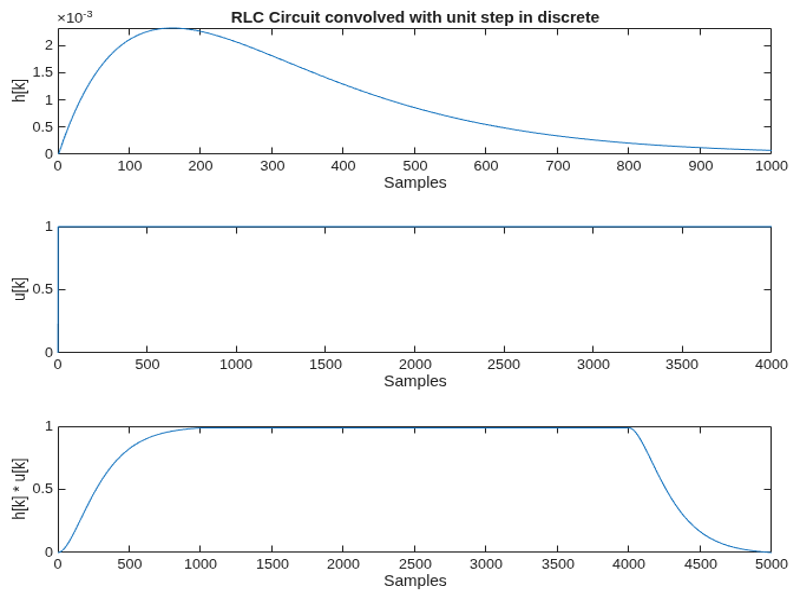
\includegraphics[scale=1]{./assets/part3/part3step4.png}
        \caption{A impulse response for an RLC circuit, unit step, and the two convoluted.}
        \label{fig:part3step4}
\end{figure}

\section*{Part 3 Step 5}
We create another vector \texttt{y2k = conv(h\_k,u2k)} using the vector \texttt{samples = 0:2999}. The plot for this is shown in figure \ref{fig:part3step5}.

\begin{figure}[H]
        \centering
        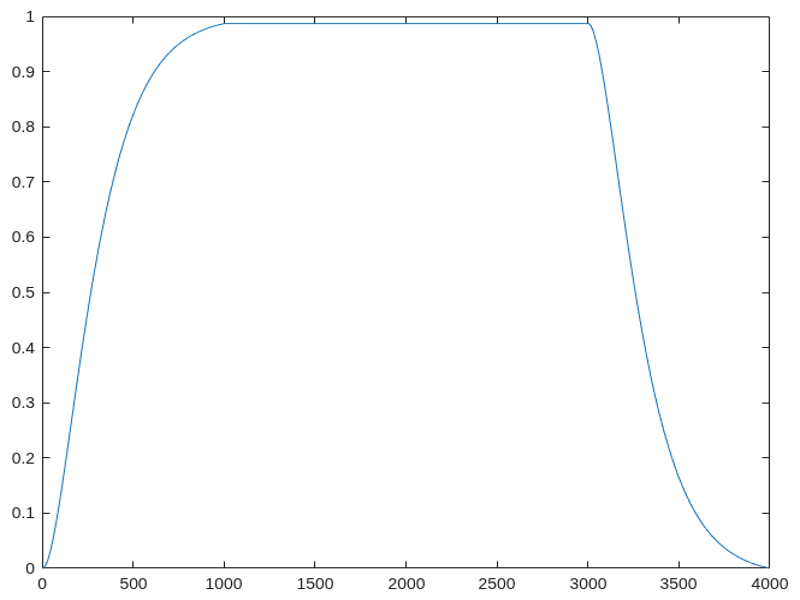
\includegraphics[scale=1]{./assets/part3/part3step5.png}
        \caption{Convolution with same size as the original unit step function.}
        \label{fig:part3step5}
\end{figure}

\section*{Part 4 Step 1}
The plot for a DSP filter is shown in figure \ref{fig:part4step3}. The \texttt{randn()} function introduces noise into the signal.
\begin{figure}[H]
	\centering
	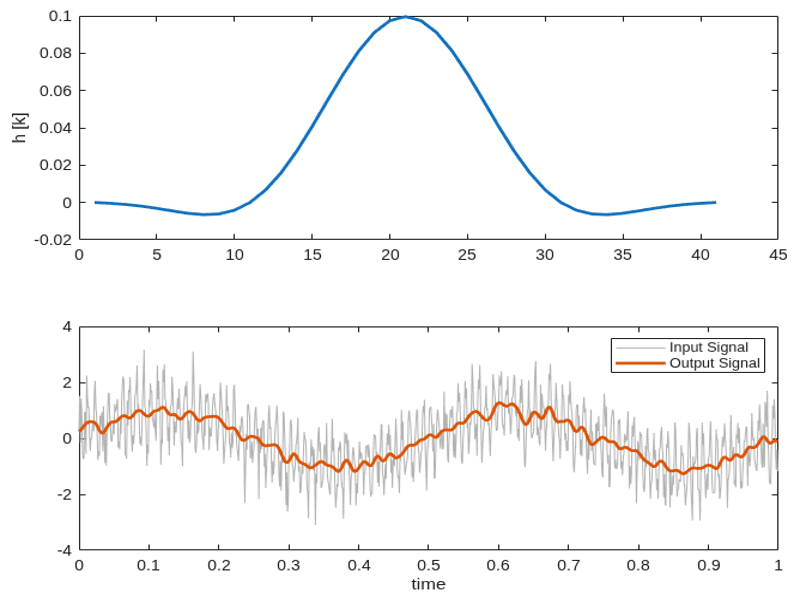
\includegraphics[scale=1]{./assets/part4/part4step3.png}
	\caption{}
	\label{fig:part4step3}
\end{figure}

\section*{Part 5 Step 1}
We first load image data using \texttt{img1=im2double(imread('tulips.png'));}.

\section*{Part 5 Step 2}
The image of the tulips is shown in figure \ref{fig:part5step2}.

\section*{Part 5 Step 3}
An image can be split into each of its color channels. The red channel is shown in figure \ref{fig:part5step3}.

\begin{figure}[H]
	\centering
	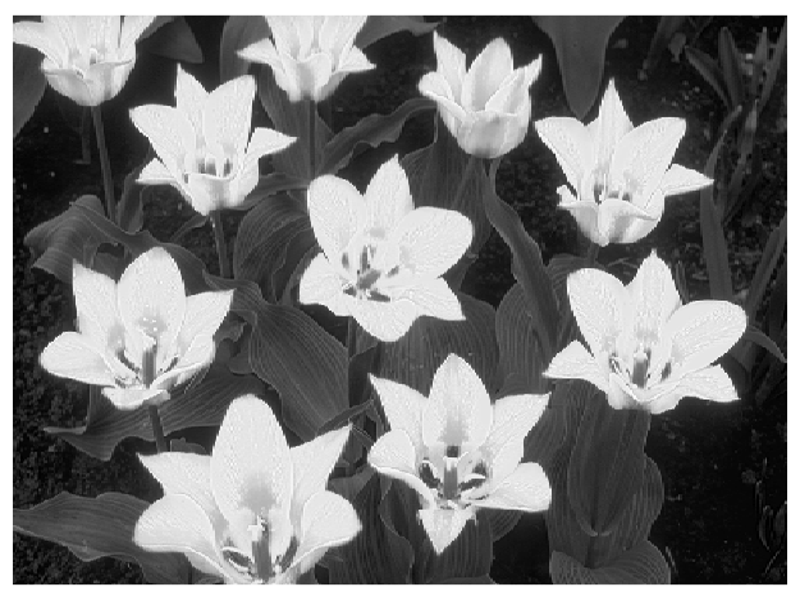
\includegraphics[scale=1]{./assets/part5/part5step3.png}
	\caption{}
	\label{fig:part5step3}
\end{figure}

\section*{Part 5 Step 4}
The green and blue channels are shown in figures \ref{fig:part5step4g} and \ref{fig:part5step4b}.

\begin{figure}[H]
	\centering
	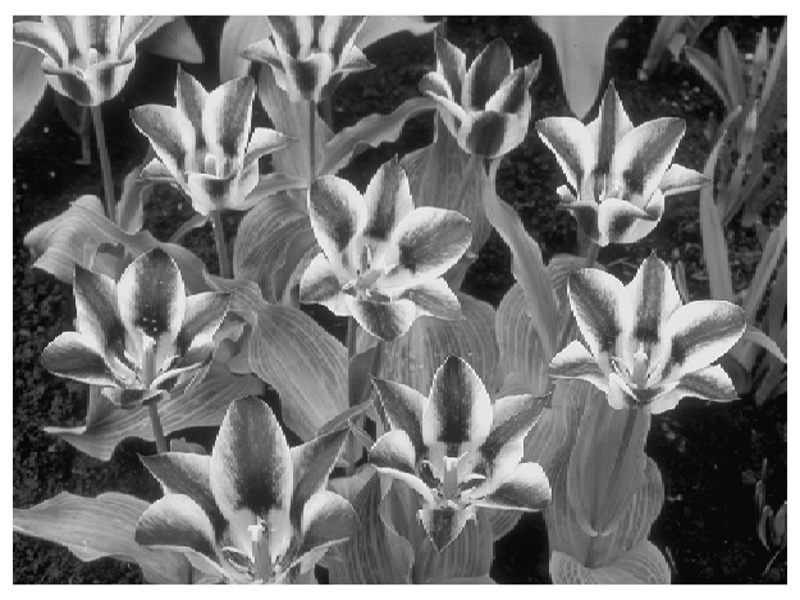
\includegraphics[scale=1]{./assets/part5/part5step4g.png}
	\caption{}
	\label{fig:part5step4g}
\end{figure}

\begin{figure}[H]
	\centering
	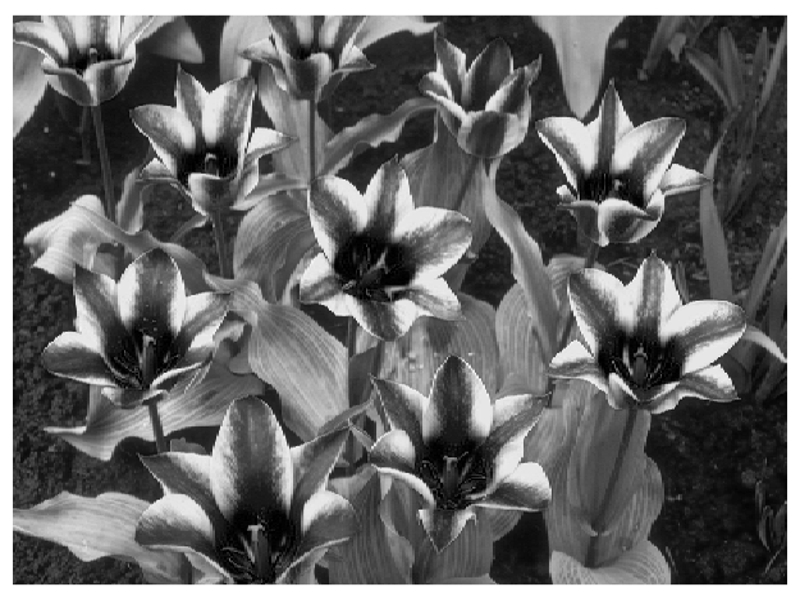
\includegraphics[scale=1]{./assets/part5/part5step4b.png}
	\caption{}
	\label{fig:part5step4b}
\end{figure}

\section*{Part 5 Step 5}
We use the kernels \texttt{h1}, \texttt{h2}, \texttt{h3}, and \texttt{h4} to manipulate the image. The first kernel will shrink the high value pixels and increase the low valued pixels effectively reducing the dynamic changes of colors. The second will boost the center pixel and subtract the surrounding. The third kernel will subtract the bottom of the center pixel from the lower half. The fourth will do the same but it will subtract the right from the left.

\section*{Part 5 Step 6}
The first kernel appears to blur the image. This makes sense because the kernel spreads the pixel values out. The second appears to sharpen the image. This makes sense because of the boosting of the center pixel. The third appears to highlight the edges of the tulips and black out everything else. The fourth appears to have the same behavior but changes the perspective. The images for these are shown in figures \ref{fig:part5step6h1}, \ref{fig:part5step6h2}, \ref{fig:part5step6h3}, and \ref{fig:part5step6h4}.

\begin{figure}[H]
	\centering
	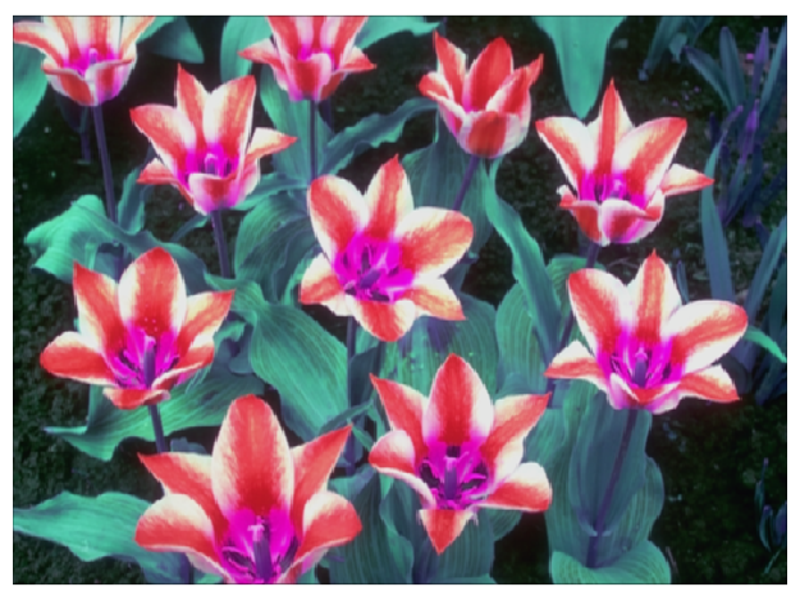
\includegraphics[scale=1]{./assets/part5/part5step6h1.png}
	\caption{}
	\label{fig:part5step6h1}
\end{figure}

\begin{figure}[H]
	\centering
	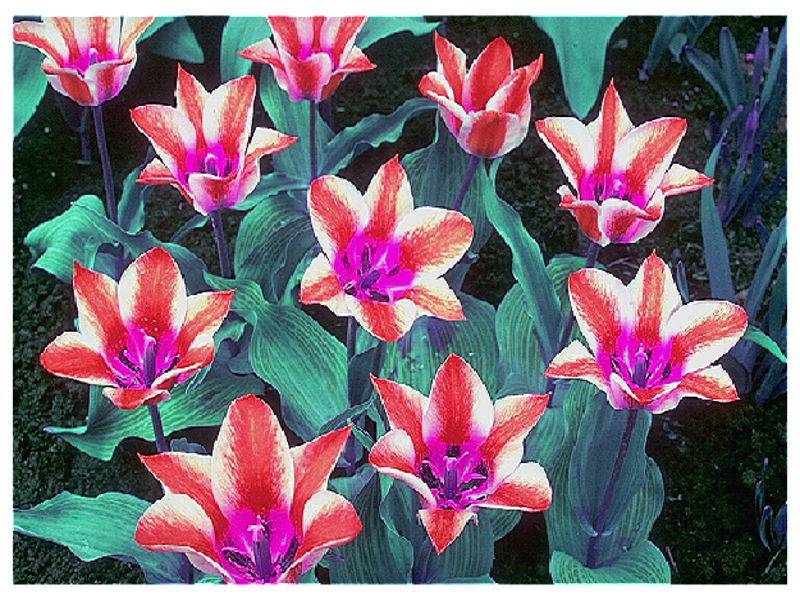
\includegraphics[scale=1]{./assets/part5/part5step6h2.png}
	\caption{}
	\label{fig:part5step6h2}
\end{figure}

\begin{figure}[H]
	\centering
	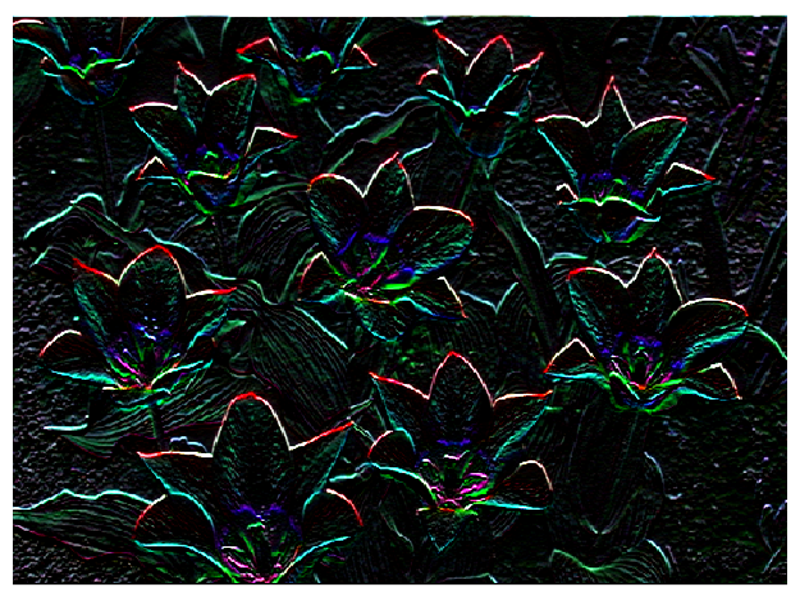
\includegraphics[scale=1]{./assets/part5/part5step6h3.png}
	\caption{}
	\label{fig:part5step6h3}
\end{figure}

\begin{figure}[H]
	\centering
	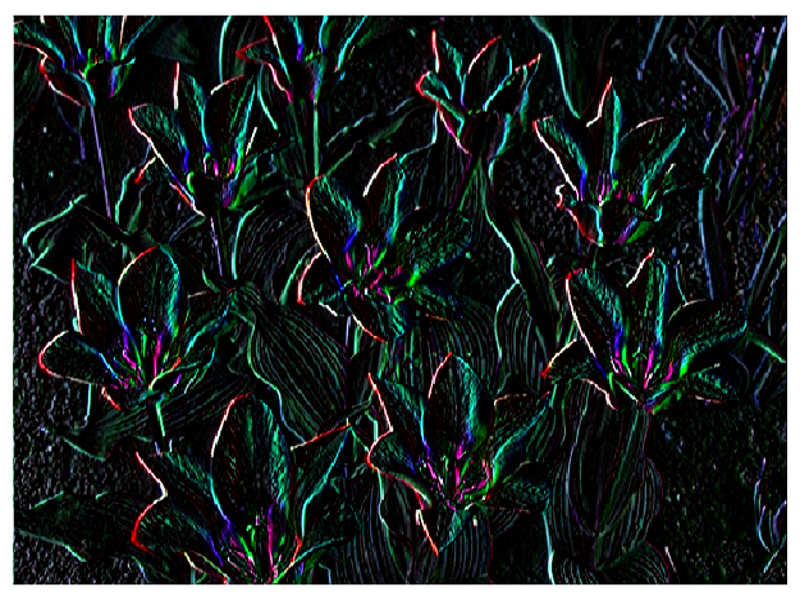
\includegraphics[scale=1]{./assets/part5/part5step6h4.png}
	\caption{}
	\label{fig:part5step6h4}
\end{figure}

%\begin{table}[H]
%	\centering
%	\begin{tabularx}{0.7\linewidth}{Y}
%	\end{tabularx}
%	\caption{}
%	\label{tab:}
%\end{table}
%\begin{figure}[H]
%        \centering
%        \includegraphics[scale=1]{./assets/}
%	\caption{}
%        \label{fig:}
%\end{figure}
\end{document}
